
%%% Local Variables: 
%%% mode: latex
%%% TeX-master: "report_dMRI_preprocessing.tex"
%%% End: 

\section{Tracking}
In the previous part~\ref{sec:reconstruction}, information about orientation of fibres at every voxel has been gained. Based on this information, we can connect these directions to reconstruct complete tracks. This processing is known as tracking, which connect voxels in order to create \emph{tracks}, or \emph{streamlines}, using the spatial information computed during the reconstruction step. An example about creating track from orientation of signal fibres within voxels is presented in figure ~\ref{Fig:tracking}

\begin{figure} 
  \centering 
  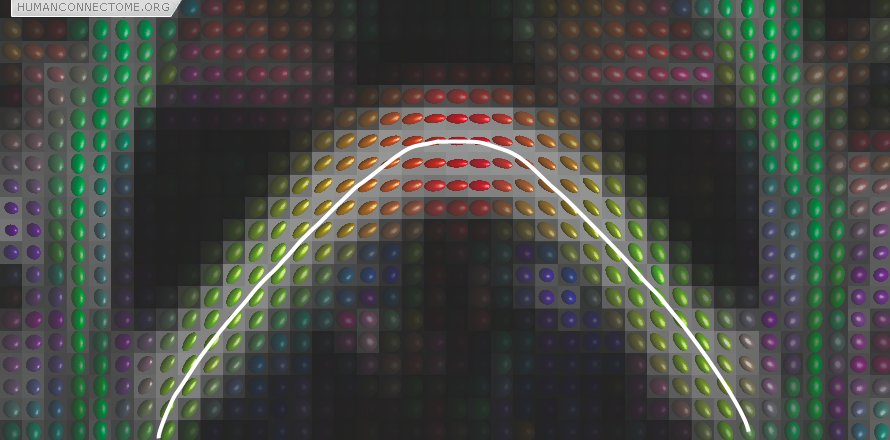
\includegraphics[width=12cm]{tensor_trajectory.jpg}
  \caption{Tracking from tensor direction information}
  \label{Fig:tracking}
\end{figure}

Brain fiber tractography is a rendering method for improving the depiction of data from diffusion imaging of the brain. Tractography is one of the most powerful tools developed to aid image interpretation. The primary purpose of tractography is to clarify the orientational architecture of tissues by integrating pathways of maximum diffusion coherence. Fibers are grown across the brain by following from voxel to voxel the direction of the diffusion maximum. The fibers depicted with tractography are often considered to represent individual axons or nerve fibers, but they are more correctly viewed in physical terms as lines of fast diffusion that follow the local diffusion maxima and that only generally reflect the axonal architecture. This distinction is useful because, for a given imaging resolution and signal-to-noise ratio, lines of maximum diffusion coherence (ie, the computer-generated fibers) may differ from the axonal architecture in some brains. Tractography adds information and interest to the MR imaging depiction of the human neuronal anatomy.

The connectivity maps obtained with tractography vary according to the diffusion imaging modality used to obtain the diffusion data. For example, diffusion tensor imaging provides a Gaussian approximation of the actual displacement distribution, and since the representation of that distribution is restricted to variations of an ellipsoid, this method creates various biases in the tractography result. In contrast, diffusion spectrum imaging with tractography overcomes many of those biases and allows more realistic mapping of connectivity. 

The application of fiber tractography to data such as those obtained with diffusion spectrum imaging or q-ball imaging results in the depiction of a large set of fiber tracts with a more complex geometry~\cite{hagmann2004diffusion}. The greater complexity obtained with this method, compared with that from tractography with diffusion tensor MR imaging data, is due to the consideration of numerous intersections between fibers that can be resolved or differentiated. 

Most tractography techniques can be grouped in three categories: local, global and simulated. Local approaches propagate a curve from a starting (seed) point using locally greedy criteria, i.e. tracking sequentially through orientation estimates in adjacent voxels. Global approaches identify the best path between two points of interest, according to some optimization criterion, rather than identifying paths arising from a single point~\cite{bihan2011MRI},~\cite{jbabdi2007bayesian}. Simulated approaches comprise of algorithms that simulate the diffusion process or solve the diffusion equation to reconstruct white matter tracks~\cite{hageman2006diffusion}~\cite{kang2005fiber}. However, solving a partial differential equation increases execution time. Furthermore, it is not always easy with these approaches to obtain a connectivity map across the whole brain volumeand there is usually a large number of parameters to set. Due to the need of creating all tractography for the whole brain, only local techniques are described in this part.

In local techniques, the two best known families of track propagation algorithms are: deterministic and probabilistic~\cite{descoteaux2009deterministic}. Deterministic fiber tracking from diffusion tensor imaging uses the principal direction of diffusion to integrate trajectories over the image~\cite{mori2002fiber} but ignores the fact that fiber orientation is often undetermined in the diffusion tensor imaging data. To overcome this limitation of the data, statistical fiber tracking methods based on consideration of the tensor as a probability distribution of fiber orientation~\cite{behrens2007probabilistic}~\cite{hagmann2003dti},~\cite{parker2003framework},~\cite{behrens2003characterization}.

In general, the deterministic algorithms propagate tracks by making a series of discrete locally optimum decisions. These are fast, simple and easy to interpret. Usually, we depict them using streamlines. A streamline is a curve that is always tangent to the velocity vector of the flow. The disadvantages of deterministic algorithms are that a pathway either exists or not (no uncertainty) and that they do not explore the entire space of possible white matter tracts. In other words, local threshold makes the tractography vulnerable to small noise aberrations. Probabilistic tractography is meant to deal with this problem of noise and propagate tracks even in regions where the tracking is unclear. This is made possible by assuming that uncertainty exists concerning the orientation of the fibre at each point of the track.

\begin{figure} 
  \centering 
  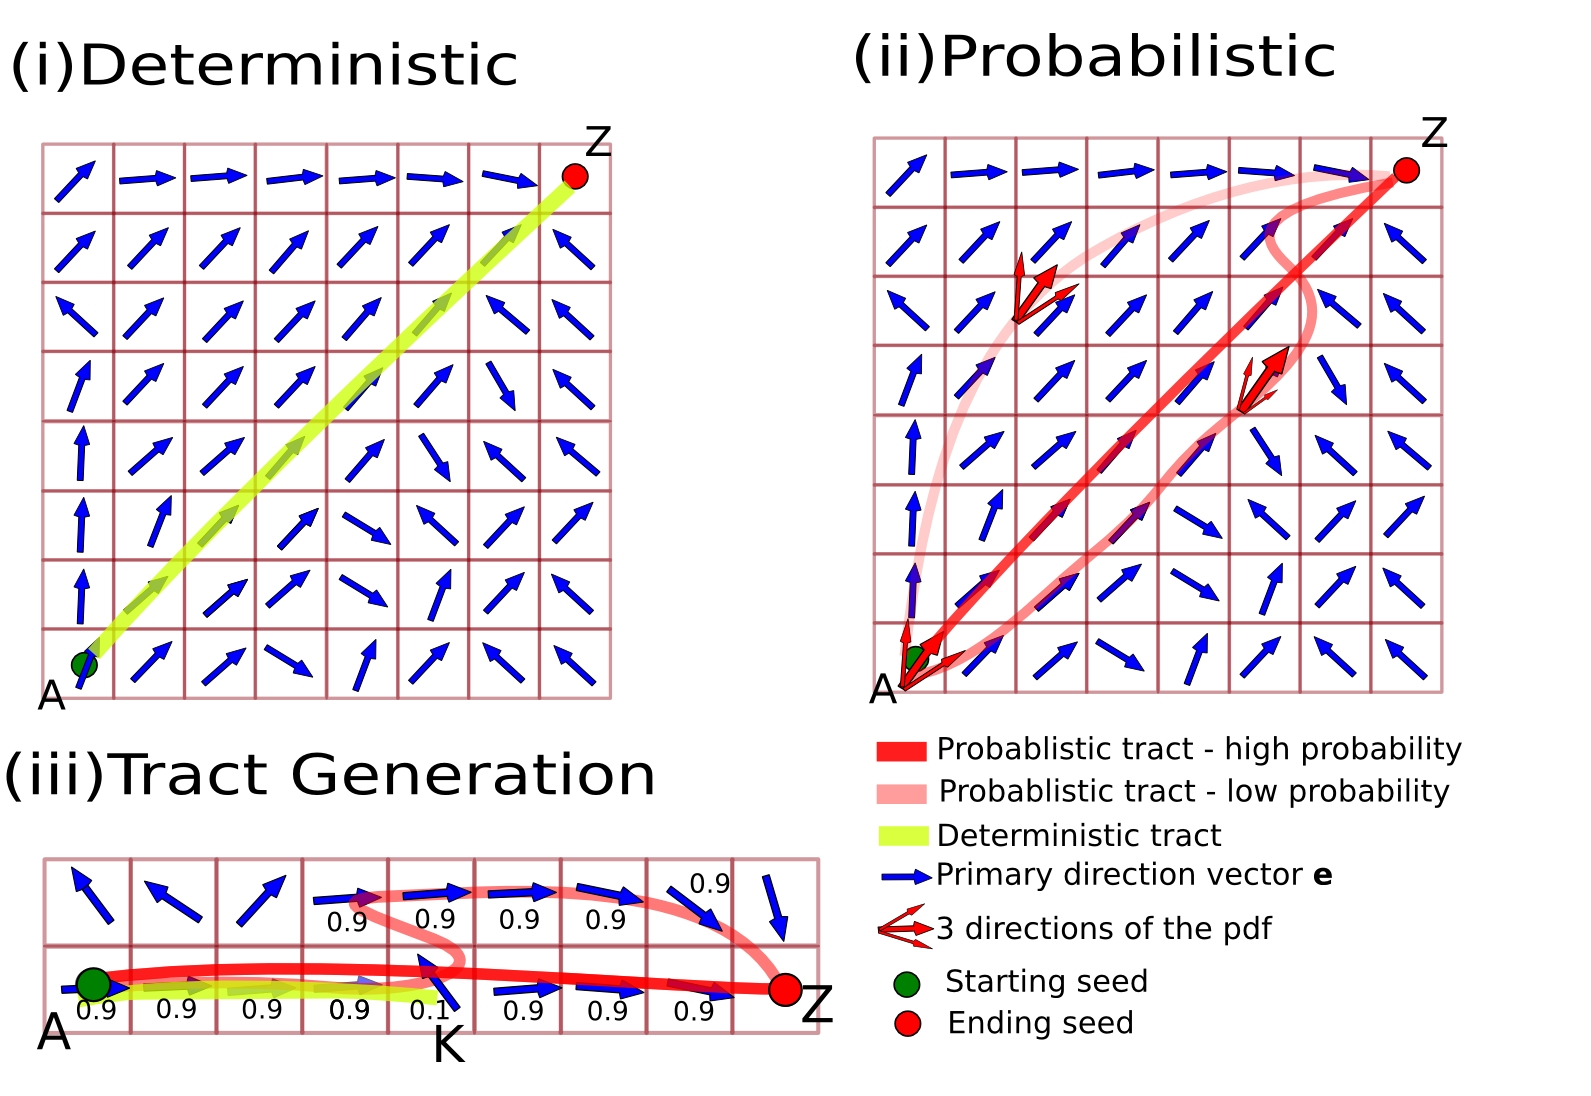
\includegraphics[width=12cm]{deterprobtrack.jpg}
  \caption{the result of deterministic and probabilistic tractography}
  \label{Fig:deterprobtrack}
\end{figure}

An example about the difference between deterministic and probabilistic is shown in the figure~\ref{Fig:deterprobtrack}. In this figure, the yellow line in (i) shows the result of deterministic tractography which is given by a single trajectory and in (ii) the tractography is given by connectivity matrix depicting with red the probability of different pathways throughout the hole slice. Here only 3 possible pathways are depicted for the ease of understanding. Finally, in (iii) an example is given where it shows that probabilistic tractography weights more closer connections. However it can tract further deep than deterministic tractography. 

When using deterministic tractography we are using only the local direction information in every pixel therefore in a direction field as this of figure~\ref{Fig:deterprobtrack}(i) we will have to use only one track and this is the diagonal pathway with yellow colour. However there are other possible tracks as well in this diagram e.g rather than taking the diagonal we could go first up north from A and then right. Probabilistic tractography aims to identify all the possible tracks by assigning to each one of them a weight. All the weights of all the tracks together sum to 1. This is possible by generating samples from a probability distribution for every pixel. In this toy example shown in figure~\ref{Fig:deterprobtrack}(ii) the orientation of the blue vectors can be represented by a single parameter, which is a random variable that takes values from a probability distribution function (PDF). Now we have many possible directions to move next but with different probabilities. The weights of all directions again sum to 1. After this explanation we can identify in figure~\ref{Fig:deterprobtrack} (ii) that the most likely track is again the diagonal (with deep red) but there are other possible tracks (with lighter red) that are less likely. In the same diagram we show with 3 combined red arrows some of the many directions that are possible in each point.

\subparagraph{EuDX-Euler integration Delta Crossing}


There are many deterministic algorithms for tracking, like FACTS~\cite{mori1999tracking} and Runge-Kutta~\cite{basser2000vivo}, PiCO. In these methods, streamlines are created as trajectories orthograde and retrograde along an initial direction at a specific point (seed) in the 3D volume. Eleftherios proposes a new method, EuDX (Euler integration Delta Crossing). EuDX is a purely deterministic method which is fast, accurate and comprehensive. But most importantly it can have as input model-based or model-free reconstruction algorithms of any known algorithm or complexity. Eu stands for Euler integration, D stands for Delta which is a function that combines together all the different stopping criteria and X stands for crossings. EuDX can deal with any number of crossings as long as your data support them. The purpose of this algorithm is to be faithful to the reconstruction results rather than try to correct or enhance them by introducing regional or global considerations which is the topic of other methods reviewed below. Therefore EuDX serves mainly as a robust method for quickly inspecting different reconstruction results using streamlines. EuDX is noise-friendly i.e. if a voxel is too noisy then EuDX will stop tracking on that voxel. This property is often useful when validating underlying orientation models. Branching is also supported by using trilinear interpolation. This method is an extension of the method used by Yeh et al. ~\cite{yeh2010qsampling} and Conturo et. al. ~\cite{conturo1999tracking} with the addition of supporting multiple anisotropic functions and multiple crossings.

\begin{equation}
  \label{eq:EuDX}
  \mathrm{EuDX}(A, D, A_{thr})
\end{equation}

where $A$, the anisotropic function, could be the FA or QA (quantitative anisotropy, from GQI) volume, $D$ represent a direction (i.e. a point on the unit sphere), and $A_{thr}$ is the anisotropy threshold. How to get these information can be found more detail in the previous section about reconstruction ~\ref{sec:reconstruction}. An example about EuDX tracking from the seed point is presented in figure~\ref{Fig:EuDXexample}

\begin{figure} 
  \centering 
  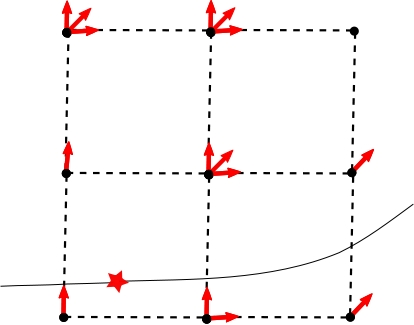
\includegraphics[width=10cm]{FDX_propagation.jpg}
  \caption{An example of EuDX tracking}
  \label{Fig:EuDXexample}
\end{figure}


The main input parameters of EuDX are:

\begin{itemize}
	\item an anisotropic scalar metric e.g. FA
        \item the indices for the peaks on the sampling sphere.
\end{itemize}

In its simplest form, this consists of starting at a seed location and following the preferred direction until we reach a new voxel. We can then change to this voxel’s referred direction and carry on until an entire track is propagated as in figure ~\ref{Fig:tracking}). Due to that, some other important options of this algorithm are:
\begin{itemize}
	\item the number of random seeds where the track propagation is initiated,
        \item a stopping criterion, for example a low threshold for anisotropy. For instance if we are using Fractional Anisotropy (FA) a typical threshold value might be $a\_low=.2$
\end{itemize}

And the syntax for calling EuDX function as below: 
\begin{python}
eu=EuDX(a=FA,ind=ten.ind(),seeds=10000,a_low=.2)
\end{python}


EuDX returns a generator class which yields a further track each time this class is called. In this way we can generate millions of tracks without using a substantial amount of memory. However, in the current example that we only have 10000 seeds, and we can load all tracks in a list using list comprehension([]) without having to worry about memory. An example of what to do for generating millions of tracks with minimum memory usage can be found on the examples directory of Dipy website~\footnote{\url{http://www.dipy.org}}. 

\begin{python}
ten_tracks=[track for track in eu]
\end{python}

In dipy we usually represent tractography as a list of tracks. Every track is a numpy array of shape (N,3) where N is the number of points in the track.

\begin{python}
print ('The number of FA tracks is %d' % len(ten_tracks))
print ('The points in ten_tracks[130] are:')
print ten_tracks[130]
\end{python}

Another way to represent tractography is as a numpy array of numpy objects. This way has an additional advantage that it can be saved very easily using numpy utilities. In theory, in a list it is faster to append an element, and in an array is faster to access. In other words both representations have different pros and cons. Other representations are possible too e.g. graphtheoretic etc.

\begin{python}
ten_tracks_asobj=np.array(ten_tracks,dtype=np.object)
np.save('ten_tracks.npy',ten_tracks_asobj)
print('FA tracks saved in ten_tracks.npy')
\end{python}

In the case there is a need to visualize the tractography, it can be easy to do by using FVTK, a module for visualization of Dipy. First, it is necessary to importe fvtk

\begin{python}
from dipy.viz import fvtk
\end{python}

Then create an instance of class \textbf{\textit{ren}} from fvtk and add tracts into this instance.

\begin{python}
renderer = fvtk.ren()
fvtk.add(renderer, fvtk.line(ten_tracks,fvtk.red,opacity=1.0))
fvtk.show(renderer)
\end{python}

Even that you want to save these tracts for using in the next time, it can be done as bellow:

\begin{python}
dpw = Dpy(<dpy_filename>, 'w')
dpw.write_tracks(ten_tracks)
dpw.close()
\end{python}
An example of tractography of subject 09 from Cambridge dataset is showed in the figure~\ref{Fig:fvtk_subj9}
\begin{figure} 
  \centering 
  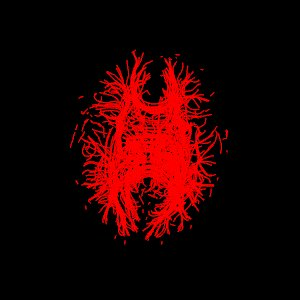
\includegraphics[width=5cm]{fvtk_subj9.jpg}
  \caption{Tractography of subject 9 from Cambridge dataset}
  \label{Fig:fvtk_subj9}
\end{figure}


In conclusion, tractography is a visualization technique that can be used to extract lines of maximum diffusion coherence from any orientation distribution function map. These lines reflect the anatomy of the axonal trajectories. Many uses are foreseen for fiber tractography, from single-tract analysis to whole-brain connectivity analysis. This part describes some common techniques for tracking. There is also a detail about the deterministic methods. At the end of this section, the EuDX algorithm is presented together the Python command line. In the next part, the last step of pre-processing of dMRI, the co-registering will be discussed.

